\noindent
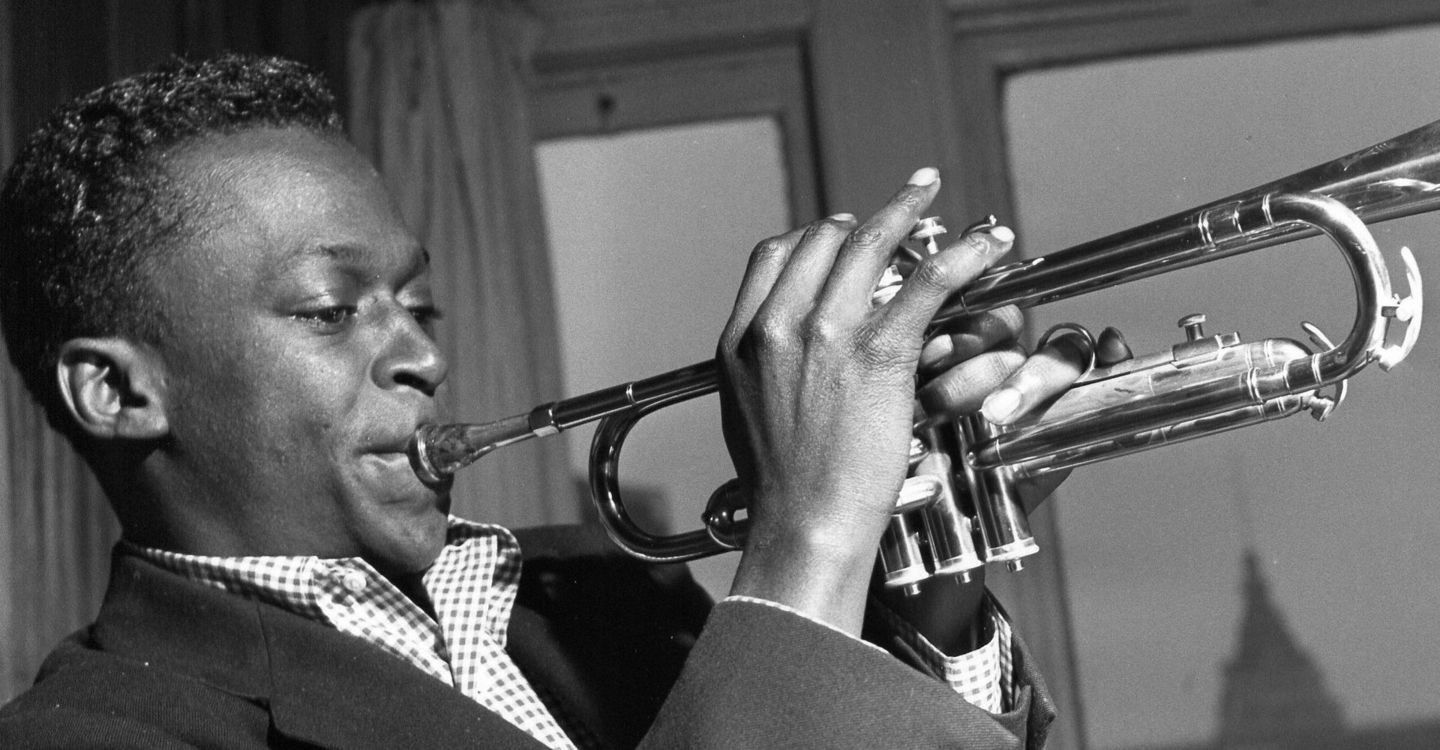
\includegraphics[width=\textwidth]{davis.jpg}

Il Jazz è un genere musicale nato negli Stati Uniti alla fine dell'Ottocento e sviluppatosi in tutto il mondo. Elemento base del jazz è l’improvvisazione. Ciò significa che i musicisti jazz non seguono una partitura, come fanno invece gli esecutori di brani di musica definita “classica”, bensì sviluppano liberamente la melodia sulla base di una progressione di accordi e di un insieme di regole ritmiche e armoniche.

Il ritmo è caratterizzato dall'uso costante del sincopato (con accenti in posizioni impreviste) e dallo "swing": una sensazione di spinta trascinante dovuta al fatto che la melodia viene percepita ora insieme, ora leggermente sfasata rispetto all'attesa scansione della misura. Le partiture scritte, quando ci sono, fungono meramente da guida, fornendo la struttura in cui inserire l'improvvisazione.
La strumentazione tipica ha come nucleo una sezione ritmica costituita da pianoforte, contrabbasso, batteria e a volte chitarra, alla quale si può aggiungere la più grande varietà di strumenti. I fiati sono raggruppati in tre sezioni: sassofoni, tromboni e trombe.

E’ un genere musicale che lascia grande libertà agli interpreti, ma che al tempo stesso richiede al jazzista una profonda conoscenza della musica e doti di grande originalità sul piano dell’esecuzione.

Durante il corso del tempo il jazz ha subito diverse variazioni ed è passato dallo swing, caratterizzato da un ritmo dondolante, al bebop, caratterizzato da tempi molto veloci.

Intorno agli anni ‘50, con l’avanzare della guerra fredda e lo scontro tra USA e URSS, negli Stati  Uniti nasce il cool Jazz, che riporta alla luce il contenuto melodico del jazz e una dimensione più rilassata delle ritmiche. Il cool jazz nasce dal desiderio di recuperare il pubblico perduto, ridando una visione e un ascolto più melodico della musica, infatti cool sta ad indicare calma, equilibrio e distacco e il più grande esponente di questa corrente jazzistica fu Miles Davis.
